\section{Hyperparameters, Features and Model Selection}
\label{app:hparams}

% Generated by scripts/paper_tables.py -- do not edit.
\typeout{[table hparams]}
\begin{table*}[t]
\centering
\footnotesize
\begin{tabular}{lp{12.5cm}}
\toprule
Setting & Value (from the run configs) \\
\midrule
GRU (v1) & proj dim 192, hidden size 128, num layers 2, input dropout 0.2, rnn dropout 0.2, head dropout 0.3 \\
CNN (v1) & channels 192, num blocks 6, kernel size 5, block dropout 0.2, head dropout 0.3 \\
Transformer (v1) & d model 192, num layers 4, num heads 4, ff dim 384, dropout 0.1, head dropout 0.3 \\
Hybrid (v2) & dim 256, num stages 3, conv blocks 2, kernel size 17, expansion dim 512, conv dropout 0.2, num heads 4, ff dim 512, attention dropout 0.1, head dropout 0.4, late dropout start 0.5 \\
v1 recipe & epochs 60, batch size 256, lr 0.001, weight decay 0.05, warmup fraction 0.05, label smoothing 0.1, grad clip 1.0, patience 15; augmentation: affine p 0.8, temporal p 0.5, jitter p 0.5 \\
v2 recipe & epochs 150, batch size 256, lr 0.0005, weight decay 0.05, warmup fraction 0.05, label smoothing 0.1, grad clip 1.0, patience 30, EMA decay 0.999; augmentation: affine p 0.8, temporal p 0.5, jitter p 0.5, rotation deg 15.0, scale min 0.85, scale max 1.15, translate 0.1, window min 0.8, jitter std 0.01, frame dropout p 0.5, time mask p 0.5, landmark mask p 0.3, hand rotation p 0.5 \\
\bottomrule
\end{tabular}
\caption{Hyperparameters, read from \cfg{experiments/train\_*.yaml} (v1) and the hybrid run's \cfg{config.yaml} (v2). Every signer-independent configuration was trained with seeds 0, 1 and 2.}
\label{tab:hparams}
\end{table*}


\paragraph{Dominant-hand mirroring.}
\label{app:mirror}
Mirroring flips \V{data.mirroredpct}\% of the Google ISLR sequences, but it is a property of
signers rather than sequences: \V{mir.high} of the \V{data.signers} signers have
more than 80\% of their sequences mirrored and \V{mir.low} have under 5\%, consistent with left-handed signers or
mirrored (selfie) recordings, which the data cannot tell apart. Every test signer is at most
\V{mir.testmax}\%.

\paragraph{Model selection.} Figure~\ref{fig:acclat} shows the candidates against the shipping
rule's latency budget (Section~\ref{sec:models}).

\begin{figure}[t]
\centering
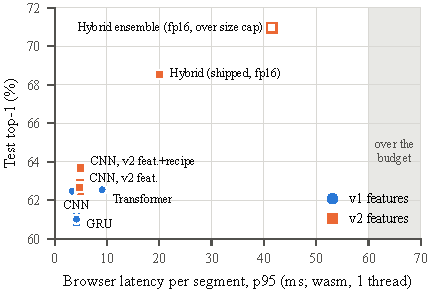
\includegraphics[width=\columnwidth]{figures/acc_latency}
\caption{Test top-1 (mean $\pm$ sd over seeds) against browser latency per call (p95, Chrome on
the i3-1115G4, wasm, one thread; selection benchmark). The hybrid ensemble is within the latency
budget but over the size cap; the single hybrid (fp16) is the most accurate model that meets both.}
\label{fig:acclat}
\end{figure}

\section{Test Signers and Test-Split Access}
\label{app:testsplit}

Table~\ref{tab:persigner} gives every signer-independent model's top-1 per Google ISLR test
signer; Table~\ref{tab:testaccess} lists every logged access to either test split, including v3's
single access to each.

% Generated by scripts/paper_tables.py -- do not edit.
\typeout{[table persigner]}
\begin{table}[t]
\centering
\footnotesize
\setlength{\tabcolsep}{3pt}
\begin{tabular}{lrrrr}
\toprule
Model & S1 & S2 & S3 & S4 \\
\midrule
CNN (v1) & 46.0 & 71.5 & 57.4 & 69.2 \\
Transformer (v1) & 46.7 & 71.4 & 55.6 & 71.1 \\
GRU (v1) & 44.7 & 70.4 & 54.7 & 68.6 \\
CNN, v2 features & 45.3 & 71.0 & 57.3 & 70.9 \\
CNN, v2 features + recipe & 45.5 & 72.2 & 58.9 & 71.6 \\
Hybrid & 51.9 & 77.7 & 61.2 & 77.6 \\
\bottomrule
\end{tabular}
\caption{Test top-1 (\%, mean over seeds) for each of the four test signers (S1--S4: 2700, 4322, 4787, 4433 sequences).}
\label{tab:persigner}
\end{table}

% Generated by scripts/paper_tables.py -- do not edit.
\typeout{[table testaccess]}
\begin{table}[t]
\centering
\footnotesize
\setlength{\tabcolsep}{3pt}
\begin{tabular}{llp{4.0cm}}
\toprule
Date (UTC) & Commit & Evaluated on test \\
\midrule
2026-11-04 & 43806b4+ & signer-dependent v1, v1 models \\
2026-11-04 & d34f874+ & quantized v1 variants \\
2026-11-06 & 3fbafa3+ & v2 models \\
2026-11-15 & 3fbafa3+ & signer-dependent v1, v1 models, v2 models \\
2026-11-16 & 36219ea+ & v1 models, v2 models, shipped ONNX file (saved logits for this paper) \\
2026-11-17 & 36219ea+ & shipped ONNX file (saved logits for this paper) \\
\bottomrule
\end{tabular}
\caption{Every logged run of the only script that reads the test split (\cfg{results/final*/test\_access\_log.json}); + marks a working tree with uncommitted changes. The v2 models were designed after the v1 evaluation in the first row.}
\label{tab:testaccess}
\end{table}


\section{ASL Citizen, v3 and Teach Dex}
\label{app:v3}

\paragraph{ASL Citizen.} Table~\ref{tab:citizen} breaks the ASL Citizen test results down by how
each label was mapped. v2 is weakest on signs mapped through a numbered variant; v3, trained on
the same mapping, is about equally accurate under all three rules, which says nothing about
whether the mapping is right. With each model's own validation temperature, v2's expected
calibration error on this split is \V{cit.v2.ece} and v3's \V{cit.v3.ece}.

\paragraph{v3 training.} v3 uses the v2 hybrid's architecture and recipe
(Table~\ref{tab:hparams}) with \V{v3.train} training and \V{v3.val} validation sequences from
\V{v3.trainsigners} and \V{v3.valsigners} signers (\V{v3.valsigners.ks} Google ISLR and
\V{v3.valsigners.cit} ASL Citizen validation signers; one of ASL Citizen's \V{cit.all.valsigners}
has no kept video of a mapped sign); its Google ISLR test split is the same as v2's.
The \V{v3.seeds} seeds scored between \V{v3.selmin}\% and \V{v3.selmax}\% on the selection
criterion, the mean of the two validation top-1 scores; a seed took about \V{v3.trainmin}
minutes on a \V{v3.gpu}.

\paragraph{Teach Dex.} The blend's weight and offset minimize the mean negative log-likelihood
over \V{td.draws} simulated draws on validation signers: in each, one signer teaches between one
and twenty-five signs with \V{td.examples} of their own sequences each, and every other sequence
of that signer is a query, taught sign or not. ASL Citizen's validation signers recorded most signs
once or twice, too few for this simulation, so v3's blend is fitted on the Google ISLR part of its
validation split, with the same draws as v2's. The blends (weight \V{td.v2.weight}, offset
\V{td.v2.offset} for v2; \V{td.v3.weight} and \V{td.v3.offset} for v3) raise validation top-1 on
taught signs from \V{td.v2.valbefore}\% to \V{td.v2.valafter}\% (v2) and from \V{td.v3.valbefore}\%
to \V{td.v3.valafter}\% (v3), and leave untaught signs where they were (\V{td.v2.valuntaught0}\%
and \V{td.v2.valuntaught1}\%; \V{td.v3.valuntaught0}\% and \V{td.v3.valuntaught1}\%).

\paragraph{The compromised v3 run of Teach Dex.} Its model-alone score on take 2,
\V{td.v3.model}\%, is far below v3's \V{lg3.web.v3.take2}\% on the same clips in the live runs of
Section~\ref{sec:liveresults} (for v2 the two agree, \V{td.v2.model}\% and \V{lg3.web.v2.take2}\%),
and its runs found ever fewer segments (\V{td.v3.segmax} down to \V{td.v3.segmin}, against
\V{td.v2.segmin}--\V{td.v2.segmax} with v2), for a reason the harness, which logs no frame rate,
cannot show. Clips without a segment cannot change, so v3's gain (\V{td.v3.diff} points, $p$ =
\V{td.v3.p}) is biased toward zero and says nothing about teaching v3.

% Generated by scripts/paper_tables.py -- do not edit.
\typeout{[table citizen]}
\begin{table}[t]
\centering
\footnotesize
\setlength{\tabcolsep}{3pt}
\begin{tabular}{lrrr}
\toprule
ASL Citizen test & Videos & v2 & v3 \\
\midrule
Top-1, exact name & \V{cit.rule.exact} & \V{cit.v2.exact} & \V{cit.v3.exact} \\
Top-1, numbered variant & \V{cit.rule.variant} & \V{cit.v2.variant} & \V{cit.v3.variant} \\
Top-1, synonym & \V{cit.rule.synonym} & \V{cit.v2.synonym} & \V{cit.v3.synonym} \\
Top-1, all & \V{cit.videos} & \V{cit.v2.top1} & \V{cit.v3.top1} \\
Top-3, all & & \V{cit.v2.top3} & \V{cit.v3.top3} \\
Top-1, range over signers & & \V{cit.v2.sigmin}--\V{cit.v2.sigmax} & \V{cit.v3.sigmin}--\V{cit.v3.sigmax} \\
\midrule
ECE, raw softmax & & \V{cit.v2.eceraw} & \V{cit.v3.eceraw} \\
ECE, temperature from val & & \V{cit.v2.ece} & \V{cit.v3.ece} \\
Coverage at val threshold & & \V{cit.v2.cov} & \V{cit.v3.cov} \\
Selective accuracy & & \V{cit.v2.sel} & \V{cit.v3.sel} \\
\bottomrule
\end{tabular}
\caption{v2 and v3 on the official ASL Citizen test split (\%, except ECE), by how the sign's label was mapped to an ASL Citizen gloss. Each model was evaluated once (\cfg{scripts/citizen\_eval.py}); the mapping is AI-assisted and unconfirmed by a signer. v3 trained on ASL Citizen's training signers.}
\label{tab:citizen}
\end{table}


\section{Calibration}
\label{app:calib}

Figure~\ref{fig:calibration} shows the deployed v2 model before and after temperature scaling.
Before scaling the model is underconfident, as a temperature below one implies
(Section~\ref{sec:models}).

\begin{figure}[t]
\centering
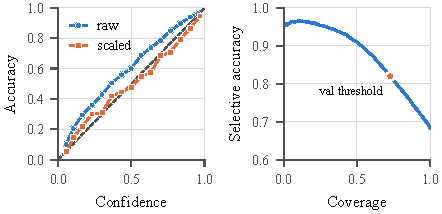
\includegraphics[width=\columnwidth]{figures/calibration}
\caption{The deployed v2 model on the Google ISLR test split. Left: reliability diagram before (raw)
and after temperature scaling (bins with at least fifty sequences); after scaling the upper bins
are slightly overconfident. Right: selective accuracy against coverage when accepting the most
confident predictions first; the dot is the threshold chosen on validation.}
\label{fig:calibration}
\end{figure}

\section{Quantization}
\label{app:quant}

Table~\ref{tab:quant} and Figure~\ref{fig:quant} give every post-training quantization variant of
the v1 models (Section~\ref{sec:efficiency}).

% Generated by scripts/paper_tables.py -- do not edit.
\typeout{[table quant]}
\begin{table}[t]
\centering
\footnotesize
\setlength{\tabcolsep}{3pt}
\begin{tabular}{llrrrr}
\toprule
Model & Variant & Top-1 & $\Delta$ & MB & p50 (ms) \\
\midrule
CNN & fp32 & 62.5 & +0.0 & 1.29 & 0.56 \\
 & fp16 & 62.5 & +0.0 & 0.67 & 0.69 \\
 & int8 dyn. & 59.3 & $-$3.1 & 0.39 & 4.78 \\
 & int8 st. & 55.7 & $-$6.8 & 0.46 & 0.64 \\
 & int8 full & 56.1 & $-$6.4 & 0.46 & 0.64 \\
\midrule
GRU & fp32 & 61.0 & +0.0 & 2.86 & 1.08 \\
 & fp16 & 61.0 & $-$0.0 & 1.44 & 1.07 \\
 & int8 dyn. & 58.4 & $-$2.7 & 2.37 & 0.99 \\
 & int8 st. & 50.6 & $-$10.4 & 2.38 & 1.02 \\
 & int8 full & 51.3 & $-$9.7 & 2.38 & 1.07 \\
\midrule
Transf. & fp32 & 62.5 & +0.0 & 5.19 & 1.56 \\
 & fp16 & 62.5 & $-$0.0 & 2.65 & 1.97 \\
 & int8 dyn. & 59.7 & $-$2.9 & 1.48 & 0.93 \\
 & int8 st. & 57.9 & $-$4.7 & 1.52 & 1.16 \\
 & int8 full & 58.6 & $-$4.0 & 1.52 & 1.39 \\
\midrule
Hybrid & fp32 & -- & -- & 13.70 & 4.10 \\
 & fp16 & -- & -- & 6.93 & 4.42 \\
 & int8 dyn. & -- & -- & 3.66 & 21.96 \\
\bottomrule
\end{tabular}
\caption{Post-training quantization of the v1 models (test top-1 \%, mean over seeds; $\Delta$ against fp32 in points) and CPU latency of one call in Python onnxruntime on the i3-1115G4 (1 intra-op thread, median p50 over three rounds, seed 0). dyn.: dynamic; st.: static with the feature block kept in float; full: static with the input and feature block quantized too. The hybrid has no int8 test evaluation (only latency and size).}
\label{tab:quant}
\end{table}


\begin{figure*}[t]
\centering
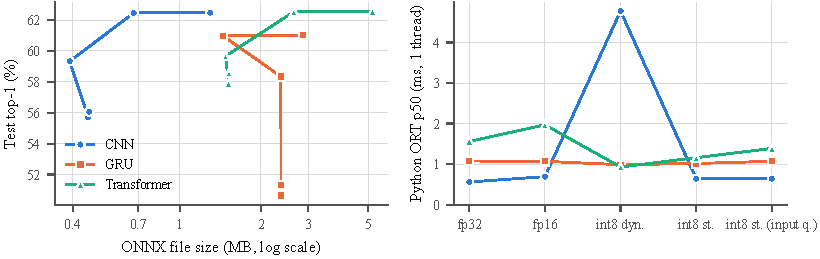
\includegraphics[width=0.9\textwidth]{figures/quant}
\caption{Post-training quantization of the v1 models. Left: test top-1 against file size (each
line runs through fp32, fp16, dynamic int8, static int8 and static int8 with the input quantized).
Right: one call in Python onnxruntime on the i3-1115G4 (1 thread, p50). Numbers are in
Table~\ref{tab:quant}.}
\label{fig:quant}
\end{figure*}

\section{Live-Gap Details}
\label{app:livegap}

\begin{figure}[t]
\centering
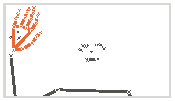
\includegraphics[width=0.6\columnwidth]{figures/skeleton}
\caption{One frame of a live clip (``hello''), drawn from its Holistic landmarks only: pose in
grey, the signer's right hand in orange. No camera image appears in this paper.}
\label{fig:skeleton}
\end{figure}

\paragraph{Segmenter.} A sign starts when a hand is present and the motion energy exceeds
\V{seg.start}, and ends when the hands are lost for \V{seg.lostms} ms, stay below \V{seg.still} for
\V{seg.stillms} ms, or after \V{seg.maxs} s; segments shorter than \V{seg.minms} ms are discarded and
gaps up to \V{seg.gapms} ms are bridged. The thresholds come from the validation sequences,
assuming their frames are \V{seg.assumedfps} fps apart: the start threshold is the
\V{seg.startpct}th percentile of the per-sequence peak energy, and the still threshold the largest
value at which at most \V{seg.stillpct}\% of sequences would be cut inside the sign.

\paragraph{Other changes.} Swapping in the hybrid before any fix gained \V{lg.web.c1model.dtop1}
points in the browser (\V{lg.web.c1model.dtop1better} clips better, none worse;
\V{lg.web.c1model.dtop1sig} at clip level, not at sign level, Holm $p$ =
\V{lg.web.c1model.dtop1psign}) and \V{lg.py.c1model.dtop1} in Python, from a floor near zero.
Resampling by time (d), which cannot matter in Python, changed browser clip top-1 by
\V{lg.web.c4time.dtop1} points, and calibration (f), which cannot change a segment's top-1, by
\V{lg.web.c6final.dtop1}. Replacing the hybrid by the v1 CNN in the final pipeline cost
\V{lg.py.xv1model.dtop1} and \V{lg.web.xv1model.dtop1} points (\V{lg.web.xv1model.dtop1sig}), so
the hybrid's test-set advantage shows only weakly here.

Figure~\ref{fig:skeleton} shows one frame of a live clip as the pipelines see it, and
Figure~\ref{fig:livegap} plots the ablation of Table~\ref{tab:livegap}.
Table~\ref{tab:livegapci} gives every live-gap configuration with its interval and its comparison
against the configuration it changes; Table~\ref{tab:persign} gives the final pipeline per sign,
next to the deployed v2 model's accuracy on the same sign in the test split. The most frequent
confusions of the final pipeline were, for Python + Holistic: \V{lg.py.confusions}; and for the
browser: \V{lg.web.confusions} (counts over takes and runs).

\begin{figure}[t]
\centering
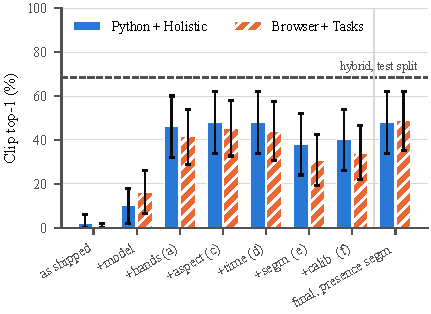
\includegraphics[width=\columnwidth]{figures/livegap}
\caption{Clip top-1 as the fixes are added one at a time, the final pipeline with presence
segmentation instead of the motion segmenter, and the hybrid's test top-1 (dashed); 95\%
bootstrap intervals over the \V{lg.clips} clips; browser bars are means over runs.}
\label{fig:livegap}
\end{figure}

% Generated by scripts/paper_tables.py -- do not edit.
\typeout{[table livegap_ci]}
\begin{table*}[t]
\centering
\footnotesize
\setlength{\tabcolsep}{2pt}
\begin{tabular}{llrrrrrrl}
\toprule
Pipeline & Config & Runs & top-1 [95\% CI] & $\Delta$ top-1 [95\% CI] & $p$ & $p_{\mathrm{Holm}}$ & $p_{\mathrm{Holm}}$, sign & Better/worse \\
\midrule
Python & As shipped (v1 CNN) & \V{lg.py.c0asshipped.runs} & \V{lg.py.c0asshipped.top1} \V{lg.py.c0asshipped.top1ci} & -- & -- & -- & -- & -- \\
Python & + v2 hybrid model & \V{lg.py.c1model.runs} & \V{lg.py.c1model.top1} \V{lg.py.c1model.top1ci} & \V{lg.py.c1model.dtop1} \V{lg.py.c1model.dtop1ci} & \V{lg.py.c1model.dtop1praw} & \V{lg.py.c1model.dtop1p} & \V{lg.py.c1model.dtop1psign} & \V{lg.py.c1model.dtop1better}/\V{lg.py.c1model.dtop1worse} \\
Python & + hand assignment (a) & \V{lg.py.c2hands.runs} & \V{lg.py.c2hands.top1} \V{lg.py.c2hands.top1ci} & \V{lg.py.c2hands.dtop1} \V{lg.py.c2hands.dtop1ci} & \V{lg.py.c2hands.dtop1praw} & \V{lg.py.c2hands.dtop1p} & \V{lg.py.c2hands.dtop1psign} & \V{lg.py.c2hands.dtop1better}/\V{lg.py.c2hands.dtop1worse} \\
Python & + aspect from frame (c) & \V{lg.py.c3aspect.runs} & \V{lg.py.c3aspect.top1} \V{lg.py.c3aspect.top1ci} & \V{lg.py.c3aspect.dtop1} \V{lg.py.c3aspect.dtop1ci} & \V{lg.py.c3aspect.dtop1praw} & \V{lg.py.c3aspect.dtop1p} & \V{lg.py.c3aspect.dtop1psign} & \V{lg.py.c3aspect.dtop1better}/\V{lg.py.c3aspect.dtop1worse} \\
Python & + time resampling (d) & \V{lg.py.c4time.runs} & \V{lg.py.c4time.top1} \V{lg.py.c4time.top1ci} & \V{lg.py.c4time.dtop1} \V{lg.py.c4time.dtop1ci} & \V{lg.py.c4time.dtop1praw} & \V{lg.py.c4time.dtop1p} & \V{lg.py.c4time.dtop1psign} & \V{lg.py.c4time.dtop1better}/\V{lg.py.c4time.dtop1worse} \\
Python & + motion segmenter (e) & \V{lg.py.c5segmenter.runs} & \V{lg.py.c5segmenter.top1} \V{lg.py.c5segmenter.top1ci} & \V{lg.py.c5segmenter.dtop1} \V{lg.py.c5segmenter.dtop1ci} & \V{lg.py.c5segmenter.dtop1praw} & \V{lg.py.c5segmenter.dtop1p} & \V{lg.py.c5segmenter.dtop1psign} & \V{lg.py.c5segmenter.dtop1better}/\V{lg.py.c5segmenter.dtop1worse} \\
Python & + calibration (f): final & \V{lg.py.c6final.runs} & \V{lg.py.c6final.top1} \V{lg.py.c6final.top1ci} & \V{lg.py.c6final.dtop1} \V{lg.py.c6final.dtop1ci} & \V{lg.py.c6final.dtop1praw} & \V{lg.py.c6final.dtop1p} & \V{lg.py.c6final.dtop1psign} & \V{lg.py.c6final.dtop1better}/\V{lg.py.c6final.dtop1worse} \\
Python & final, old hand mapping & \V{lg.py.xhands.runs} & \V{lg.py.xhands.top1} \V{lg.py.xhands.top1ci} & \V{lg.py.xhands.dtop1} \V{lg.py.xhands.dtop1ci} & \V{lg.py.xhands.dtop1praw} & \V{lg.py.xhands.dtop1p} & \V{lg.py.xhands.dtop1psign} & \V{lg.py.xhands.dtop1better}/\V{lg.py.xhands.dtop1worse} \\
Python & final, no aspect corr. & \V{lg.py.xaspectoff.runs} & \V{lg.py.xaspectoff.top1} \V{lg.py.xaspectoff.top1ci} & \V{lg.py.xaspectoff.dtop1} \V{lg.py.xaspectoff.dtop1ci} & \V{lg.py.xaspectoff.dtop1praw} & \V{lg.py.xaspectoff.dtop1p} & \V{lg.py.xaspectoff.dtop1psign} & \V{lg.py.xaspectoff.dtop1better}/\V{lg.py.xaspectoff.dtop1worse} \\
Python & final, body-ratio aspect & \V{lg.py.xaspectcalibrated.runs} & \V{lg.py.xaspectcalibrated.top1} \V{lg.py.xaspectcalibrated.top1ci} & \V{lg.py.xaspectcalibrated.dtop1} \V{lg.py.xaspectcalibrated.dtop1ci} & \V{lg.py.xaspectcalibrated.dtop1praw} & \V{lg.py.xaspectcalibrated.dtop1p} & \V{lg.py.xaspectcalibrated.dtop1psign} & \V{lg.py.xaspectcalibrated.dtop1better}/\V{lg.py.xaspectcalibrated.dtop1worse} \\
Python & final, index resampling & \V{lg.py.xindex.runs} & \V{lg.py.xindex.top1} \V{lg.py.xindex.top1ci} & \V{lg.py.xindex.dtop1} \V{lg.py.xindex.dtop1ci} & \V{lg.py.xindex.dtop1praw} & \V{lg.py.xindex.dtop1p} & \V{lg.py.xindex.dtop1psign} & \V{lg.py.xindex.dtop1better}/\V{lg.py.xindex.dtop1worse} \\
Python & final, presence segmenter & \V{lg.py.xpresence.runs} & \V{lg.py.xpresence.top1} \V{lg.py.xpresence.top1ci} & \V{lg.py.xpresence.dtop1} \V{lg.py.xpresence.dtop1ci} & \V{lg.py.xpresence.dtop1praw} & \V{lg.py.xpresence.dtop1p} & \V{lg.py.xpresence.dtop1psign} & \V{lg.py.xpresence.dtop1better}/\V{lg.py.xpresence.dtop1worse} \\
Python & final, v1 CNN & \V{lg.py.xv1model.runs} & \V{lg.py.xv1model.top1} \V{lg.py.xv1model.top1ci} & \V{lg.py.xv1model.dtop1} \V{lg.py.xv1model.dtop1ci} & \V{lg.py.xv1model.dtop1praw} & \V{lg.py.xv1model.dtop1p} & \V{lg.py.xv1model.dtop1psign} & \V{lg.py.xv1model.dtop1better}/\V{lg.py.xv1model.dtop1worse} \\
\midrule
Browser & Shipped build & \V{lg.web.c0headbuild.runs} & \V{lg.web.c0headbuild.top1} \V{lg.web.c0headbuild.top1ci} & -- & -- & -- & -- & -- \\
Browser & As shipped (v1 CNN) & \V{lg.web.c0asshipped.runs} & \V{lg.web.c0asshipped.top1} \V{lg.web.c0asshipped.top1ci} & -- & -- & -- & -- & -- \\
Browser & + v2 hybrid model & \V{lg.web.c1model.runs} & \V{lg.web.c1model.top1} \V{lg.web.c1model.top1ci} & \V{lg.web.c1model.dtop1} \V{lg.web.c1model.dtop1ci} & \V{lg.web.c1model.dtop1praw} & \V{lg.web.c1model.dtop1p} & \V{lg.web.c1model.dtop1psign} & \V{lg.web.c1model.dtop1better}/\V{lg.web.c1model.dtop1worse} \\
Browser & + hand assignment (a) & \V{lg.web.c2hands.runs} & \V{lg.web.c2hands.top1} \V{lg.web.c2hands.top1ci} & \V{lg.web.c2hands.dtop1} \V{lg.web.c2hands.dtop1ci} & \V{lg.web.c2hands.dtop1praw} & \V{lg.web.c2hands.dtop1p} & \V{lg.web.c2hands.dtop1psign} & \V{lg.web.c2hands.dtop1better}/\V{lg.web.c2hands.dtop1worse} \\
Browser & + aspect from frame (c) & \V{lg.web.c3aspect.runs} & \V{lg.web.c3aspect.top1} \V{lg.web.c3aspect.top1ci} & \V{lg.web.c3aspect.dtop1} \V{lg.web.c3aspect.dtop1ci} & \V{lg.web.c3aspect.dtop1praw} & \V{lg.web.c3aspect.dtop1p} & \V{lg.web.c3aspect.dtop1psign} & \V{lg.web.c3aspect.dtop1better}/\V{lg.web.c3aspect.dtop1worse} \\
Browser & + time resampling (d) & \V{lg.web.c4time.runs} & \V{lg.web.c4time.top1} \V{lg.web.c4time.top1ci} & \V{lg.web.c4time.dtop1} \V{lg.web.c4time.dtop1ci} & \V{lg.web.c4time.dtop1praw} & \V{lg.web.c4time.dtop1p} & \V{lg.web.c4time.dtop1psign} & \V{lg.web.c4time.dtop1better}/\V{lg.web.c4time.dtop1worse} \\
Browser & + motion segmenter (e) & \V{lg.web.c5segmenter.runs} & \V{lg.web.c5segmenter.top1} \V{lg.web.c5segmenter.top1ci} & \V{lg.web.c5segmenter.dtop1} \V{lg.web.c5segmenter.dtop1ci} & \V{lg.web.c5segmenter.dtop1praw} & \V{lg.web.c5segmenter.dtop1p} & \V{lg.web.c5segmenter.dtop1psign} & \V{lg.web.c5segmenter.dtop1better}/\V{lg.web.c5segmenter.dtop1worse} \\
Browser & + calibration (f): final & \V{lg.web.c6final.runs} & \V{lg.web.c6final.top1} \V{lg.web.c6final.top1ci} & \V{lg.web.c6final.dtop1} \V{lg.web.c6final.dtop1ci} & \V{lg.web.c6final.dtop1praw} & \V{lg.web.c6final.dtop1p} & \V{lg.web.c6final.dtop1psign} & \V{lg.web.c6final.dtop1better}/\V{lg.web.c6final.dtop1worse} \\
Browser & final, old hand mapping & \V{lg.web.xhands.runs} & \V{lg.web.xhands.top1} \V{lg.web.xhands.top1ci} & \V{lg.web.xhands.dtop1} \V{lg.web.xhands.dtop1ci} & \V{lg.web.xhands.dtop1praw} & \V{lg.web.xhands.dtop1p} & \V{lg.web.xhands.dtop1psign} & \V{lg.web.xhands.dtop1better}/\V{lg.web.xhands.dtop1worse} \\
Browser & final, mirrored frame (b) & \V{lg.web.xmirrored.runs} & \V{lg.web.xmirrored.top1} \V{lg.web.xmirrored.top1ci} & \V{lg.web.xmirrored.dtop1} \V{lg.web.xmirrored.dtop1ci} & \V{lg.web.xmirrored.dtop1praw} & \V{lg.web.xmirrored.dtop1p} & \V{lg.web.xmirrored.dtop1psign} & \V{lg.web.xmirrored.dtop1better}/\V{lg.web.xmirrored.dtop1worse} \\
Browser & final, mirrored + old mapping & \V{lg.web.xmirroredlabel.runs} & \V{lg.web.xmirroredlabel.top1} \V{lg.web.xmirroredlabel.top1ci} & \V{lg.web.xmirroredlabel.dtop1} \V{lg.web.xmirroredlabel.dtop1ci} & \V{lg.web.xmirroredlabel.dtop1praw} & \V{lg.web.xmirroredlabel.dtop1p} & \V{lg.web.xmirroredlabel.dtop1psign} & \V{lg.web.xmirroredlabel.dtop1better}/\V{lg.web.xmirroredlabel.dtop1worse} \\
Browser & final, no aspect corr. & \V{lg.web.xaspectoff.runs} & \V{lg.web.xaspectoff.top1} \V{lg.web.xaspectoff.top1ci} & \V{lg.web.xaspectoff.dtop1} \V{lg.web.xaspectoff.dtop1ci} & \V{lg.web.xaspectoff.dtop1praw} & \V{lg.web.xaspectoff.dtop1p} & \V{lg.web.xaspectoff.dtop1psign} & \V{lg.web.xaspectoff.dtop1better}/\V{lg.web.xaspectoff.dtop1worse} \\
Browser & final, body-ratio aspect & \V{lg.web.xaspectcalibrated.runs} & \V{lg.web.xaspectcalibrated.top1} \V{lg.web.xaspectcalibrated.top1ci} & \V{lg.web.xaspectcalibrated.dtop1} \V{lg.web.xaspectcalibrated.dtop1ci} & \V{lg.web.xaspectcalibrated.dtop1praw} & \V{lg.web.xaspectcalibrated.dtop1p} & \V{lg.web.xaspectcalibrated.dtop1psign} & \V{lg.web.xaspectcalibrated.dtop1better}/\V{lg.web.xaspectcalibrated.dtop1worse} \\
Browser & final, index resampling & \V{lg.web.xindex.runs} & \V{lg.web.xindex.top1} \V{lg.web.xindex.top1ci} & \V{lg.web.xindex.dtop1} \V{lg.web.xindex.dtop1ci} & \V{lg.web.xindex.dtop1praw} & \V{lg.web.xindex.dtop1p} & \V{lg.web.xindex.dtop1psign} & \V{lg.web.xindex.dtop1better}/\V{lg.web.xindex.dtop1worse} \\
Browser & final, presence segmenter & \V{lg.web.xpresence.runs} & \V{lg.web.xpresence.top1} \V{lg.web.xpresence.top1ci} & \V{lg.web.xpresence.dtop1} \V{lg.web.xpresence.dtop1ci} & \V{lg.web.xpresence.dtop1praw} & \V{lg.web.xpresence.dtop1p} & \V{lg.web.xpresence.dtop1psign} & \V{lg.web.xpresence.dtop1better}/\V{lg.web.xpresence.dtop1worse} \\
Browser & final, v1 CNN & \V{lg.web.xv1model.runs} & \V{lg.web.xv1model.top1} \V{lg.web.xv1model.top1ci} & \V{lg.web.xv1model.dtop1} \V{lg.web.xv1model.dtop1ci} & \V{lg.web.xv1model.dtop1praw} & \V{lg.web.xv1model.dtop1p} & \V{lg.web.xv1model.dtop1psign} & \V{lg.web.xv1model.dtop1better}/\V{lg.web.xv1model.dtop1worse} \\
\bottomrule
\end{tabular}
\caption{The live study in full: clip-level accuracy (\%) with percentile bootstrap intervals over the \V{lg.clips} clips, and each config against the config it changes: paired bootstrap interval of the difference (points, not adjusted for multiplicity), the sign-flip $p$ before and after Holm adjustment within the pipeline (the pre-specified analysis), the Holm-adjusted $p$ with the two takes of a sign as one unit (a sensitivity analysis), and the number of clips that got better/worse. Runs: browser runs averaged per configuration.}
\label{tab:livegapci}
\end{table*}

% Generated by scripts/paper_tables.py -- do not edit.
\typeout{[table persign]}
\begin{table*}[t]
\centering
\footnotesize
\setlength{\tabcolsep}{3pt}
\begin{tabular}{lrrr>{\raggedright\arraybackslash}p{5.5cm}>{\raggedright\arraybackslash}p{5.5cm}}
\toprule
Sign & Python & Browser & Test & Python predictions & Browser predictions \\
\midrule
bed & 100 & 100 & 66 & bed x2 & bed x6 \\
bird & 0 & 0 & 90 & loud x1, awake x1 & no segment x6 \\
book & 50 & 0 & 40 & book x1, no segment x1 & no segment x5, puzzle x1 \\
car & 50 & 33 & 78 & fast x1, car x1 & weus x2, fast x2, car x2 \\
cat & 50 & 33 & 57 & hair x1, cat x1 & hair x2, kitty x2, cat x2 \\
dad & 0 & 0 & 96 & donkey x2 & donkey x6 \\
dog & 100 & 50 & 61 & dog x2 & dog x3, no segment x3 \\
drink & 50 & 33 & 78 & look x1, drink x1 & look x4, drink x2 \\
finish & 0 & 0 & 67 & fine x1, noisy x1 & dog x3, cat x3 \\
food & 50 & 50 & 82 & kiss x1, food x1 & morning x3, food x3 \\
go & 0 & 0 & 30 & green x2 & green x4, moon x2 \\
happy & 0 & 0 & 81 & no segment x1, all x1 & no segment x6 \\
hello & 100 & 100 & 82 & hello x2 & hello x6 \\
home & 100 & 100 & 92 & home x2 & home x6 \\
hungry & 0 & 0 & 86 & giraffe x1, no segment x1 & giraffe x2, no segment x2, any x2 \\
milk & 100 & 100 & 77 & milk x2 & milk x6 \\
mom & 50 & 0 & 73 & mom x1, no segment x1 & no segment x3, bed x2, quiet x1 \\
no & 50 & 0 & 72 & read x1, no x1 & read x3, horse x2, uncle x1 \\
please & 50 & 100 & 93 & please x1, before x1 & please x6 \\
read & 0 & 17 & 57 & dog x1, flag x1 & arm x2, jump x2, open x1, read x1 \\
sad & 0 & 0 & 88 & mitten x1, zipper x1 & sticky x3, mitten x3 \\
sleep & 50 & 50 & 70 & sleep x1, sleepy x1 & sleep x3, sleepy x3 \\
thankyou & 0 & 0 & 75 & no segment x2 & no segment x6 \\
water & 0 & 0 & 89 & no segment x1, dirty x1 & talk x2, bedroom x1, grass x1, after x1, no segment x1 \\
yes & 50 & 83 & 42 & can x1, yes x1 & yes x5, can x1 \\
\bottomrule
\end{tabular}
\caption{Per sign, final pipeline: live clip top-1 (\%) over the two takes in Python and in the browser (and its runs), the deployed v2 model's top-1 (\%, Test) on the same sign in the test split, and the clip-level predictions with counts (``no segment'': no classified segment in the clip). Generated from \cfg{results/live\_gap\_v2/summary.json}.}
\label{tab:persign}
\end{table*}


\section{Pilot: Ten Screen-Recorded Clips}
\label{app:pilot}

Before the main live test, a pilot used ten clips, one per sign with several repetitions each,
recorded as screen captures of the first version of the demo. Two pairs of these files turned out
to be byte-identical (``yes'' = ``no'', ``dad'' = ``mom''), so one clip of each pair necessarily
carries a wrong label. We exclude all four from every statistic and report only the six
unambiguous clips (Table~\ref{tab:pilot}), without intervals: with six clips, one clip moves
accuracy by about seventeen points. The pilot motivated the fixes and their order; nothing was
tuned on it, and the main evaluation uses new recordings.

% Generated by scripts/paper_tables.py -- do not edit.
\typeout{[table pilot]}
\begin{table}[t]
\centering
\small
\setlength{\tabcolsep}{3pt}
\begin{tabular}{lrr}
\toprule
Config & Python & Browser \\
\midrule
Shipped build & --/6 & 0/6 \\
As shipped (v1 CNN) & 0/6 & 0/6 \\
+ v2 hybrid model & 2/6 & 2/6 \\
+ hand assignment (a) & 4/6 & 6/6 \\
+ aspect from frame (c) & 4/6 & 6/6 \\
+ time resampling (d) & 4/6 & 6/6 \\
+ motion segmenter (e) & 5/6 & 4/6 \\
+ calibration (f): final & 5/6 & 5/6 \\
\bottomrule
\end{tabular}
\caption{Pilot: clips correct (clip-level top-1) among the six pilot clips that are not byte-identical duplicates; the two duplicate pairs are excluded. Browser rows are means over one to three runs (Appendix~\ref{app:pilot}).}
\label{tab:pilot}
\end{table}


\section{Reproducibility}
\label{app:repro}

Code, configurations and every result file read by the paper's generators are in the project
repository; \cfg{paper/README.md} lists the commands. The paper's tables, numbers and figures are
written by \cfg{scripts/paper\_tables.py} and \cfg{scripts/paper\_figures.py} from those files, and
\cfg{scripts/paper\_claims.py} re-reads every number from its source (\cfg{paper/CLAIMS.md}).
Training ran on Kaggle (\V{m.gpu}, code at commit \V{repro.train}; v3 at commit \V{v3.commit},
in private notebooks); the test predictions, CPU benchmark and live evaluations ran on the
i3-1115G4 laptop from commit \V{repro.base} (v3's from \V{v3.commit}) with the evaluation scripts
that are committed together with this paper. The live clips and both datasets are not
redistributed, and neither is v3, which ASL Citizen's license keeps private. The web app is a
static site: a service worker caches the model for offline use and adds the cross-origin isolation
headers that WebAssembly threads need on static hosting.
